\section{Ejemplo 4}

    \lipsum[1]
    
    \begin{figure}[h]
    	\centering
    	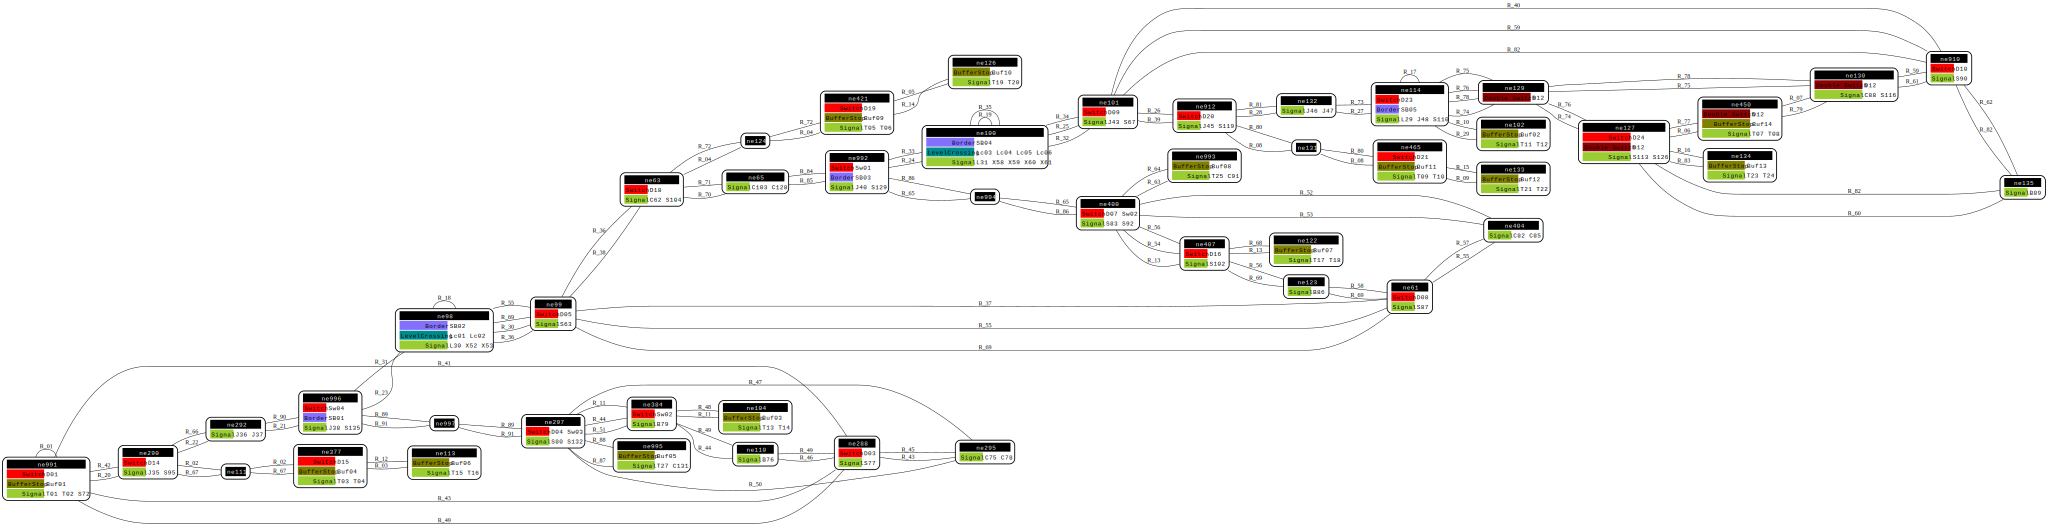
\includegraphics[width=1\textwidth]{Figuras/Graph_4}
    	\centering\caption{XXXX}
    	%\label{fig:LC_P2}
    \end{figure}
    
    \lipsum[1]

    \begin{figure}[h]
        \centering
        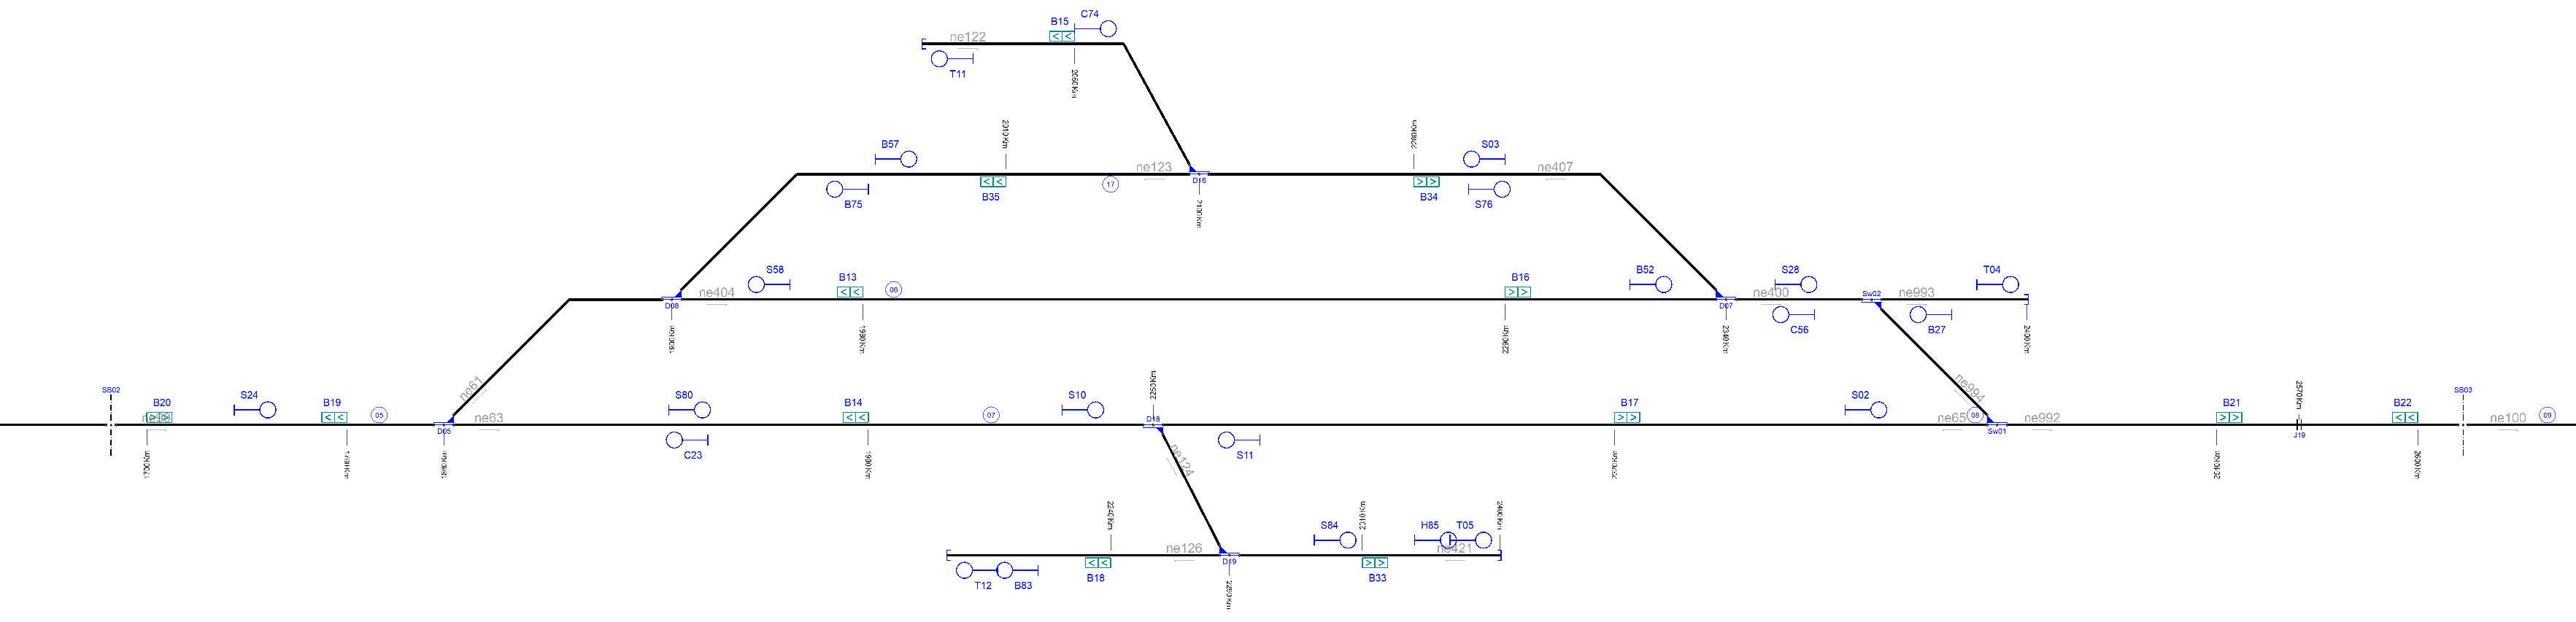
\includegraphics[width=1\textwidth]{resultados-obtenidos/ejemplo4/images/4_original.png}
        \centering\caption{Señalamiento original del ejemplo 4.}
        %\label{fig:LC_P2}
    \end{figure}

    \lipsum[1]
    
    \begin{figure}[h]
        \centering
        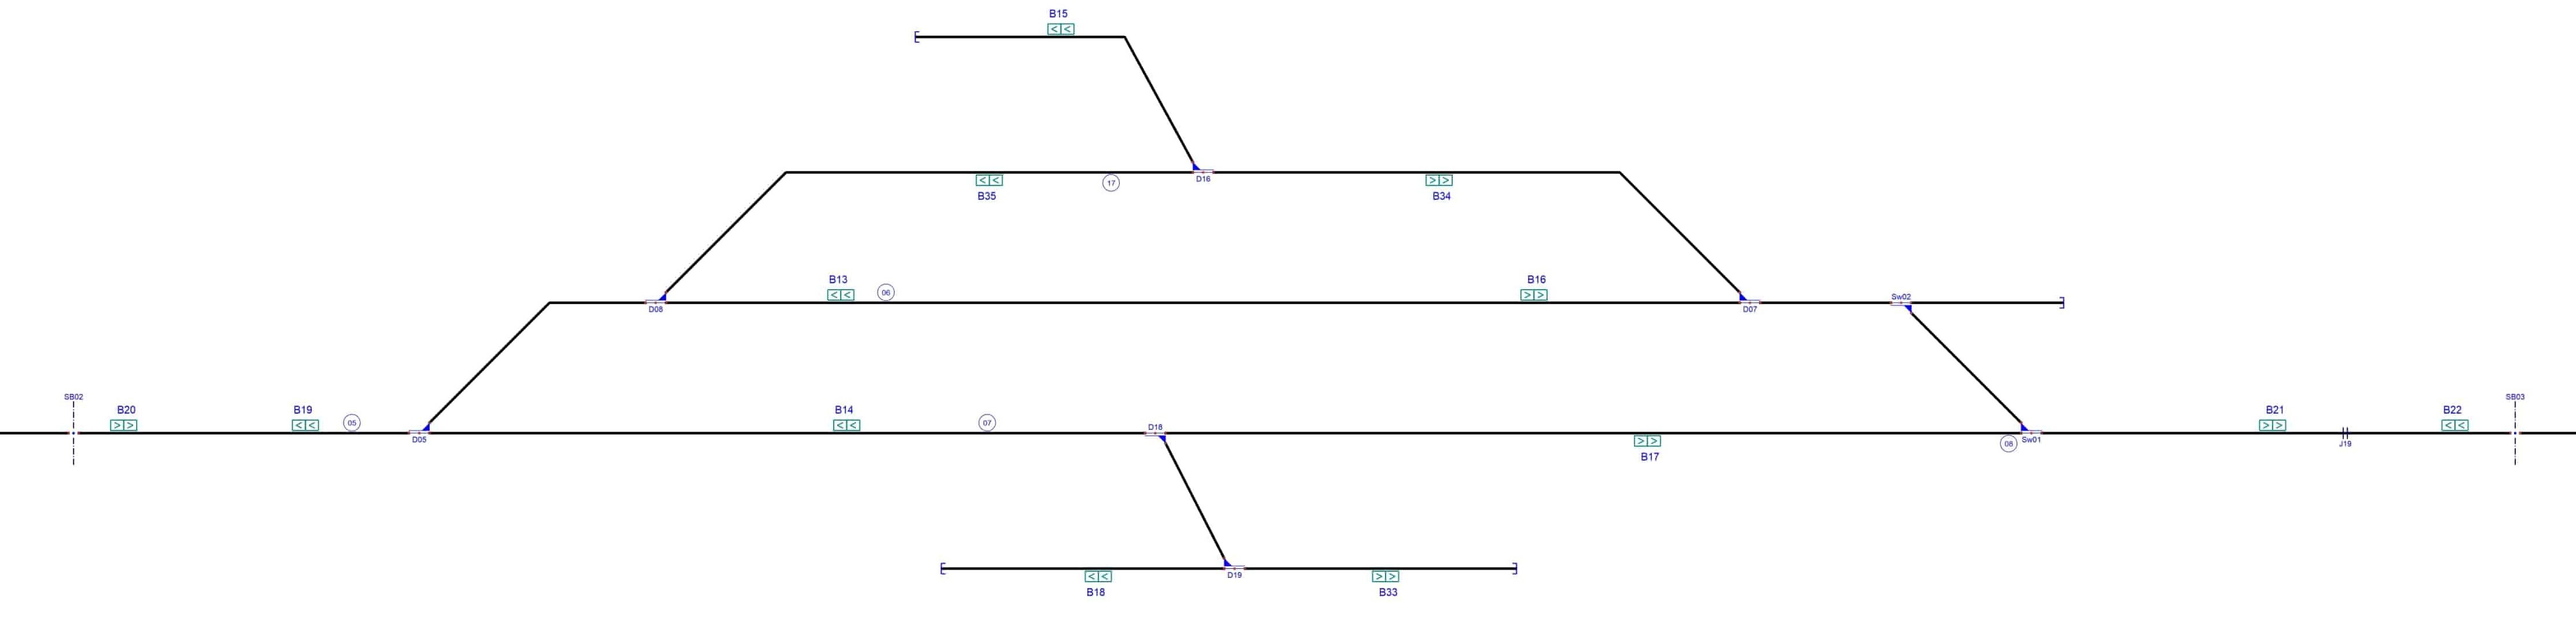
\includegraphics[width=1\textwidth]{resultados-obtenidos/ejemplo4/images/4_empty.png}
        \centering\caption{Topología ferroviaria del ejemplo 4 sin señalamiento.}
        %\label{fig:LC_P2}
    \end{figure}

    \begin{figure}[h]
        \centering
        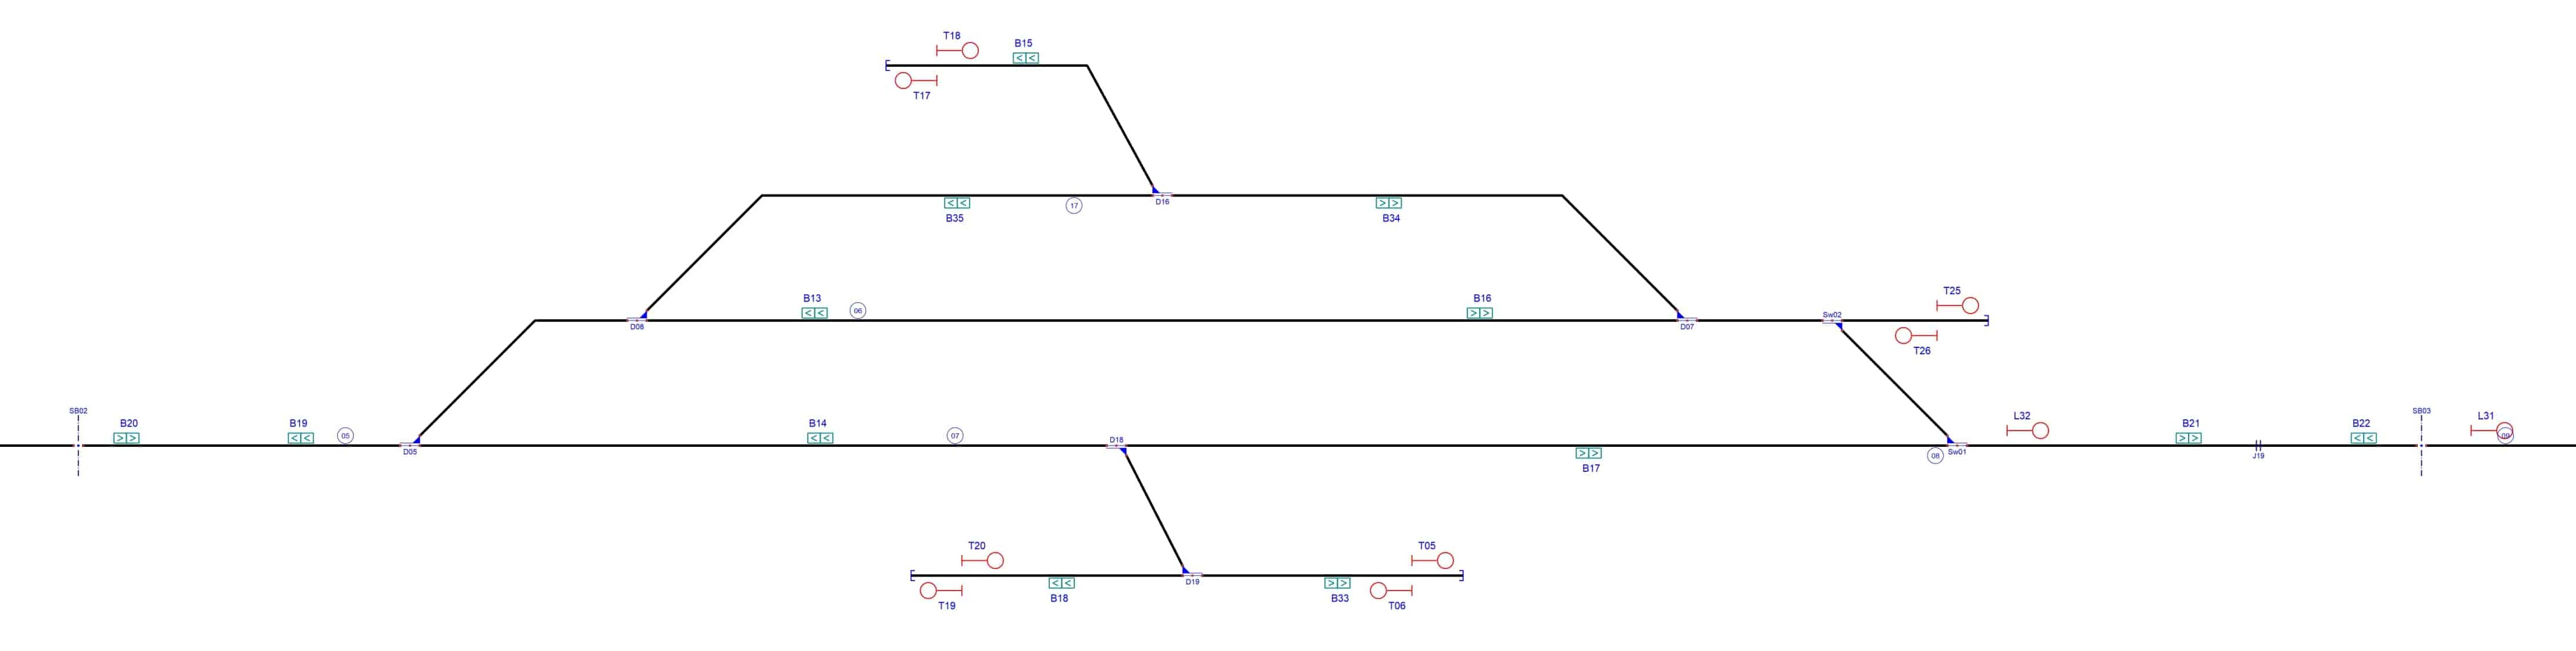
\includegraphics[width=1\textwidth]{resultados-obtenidos/ejemplo4/images/4_step1.png}
        \centering\caption{Señalamiento generado por el RNA para proteger el fín de vía.}
        %\label{fig:LC_P2}
    \end{figure}

    \begin{figure}[h]
        \centering
        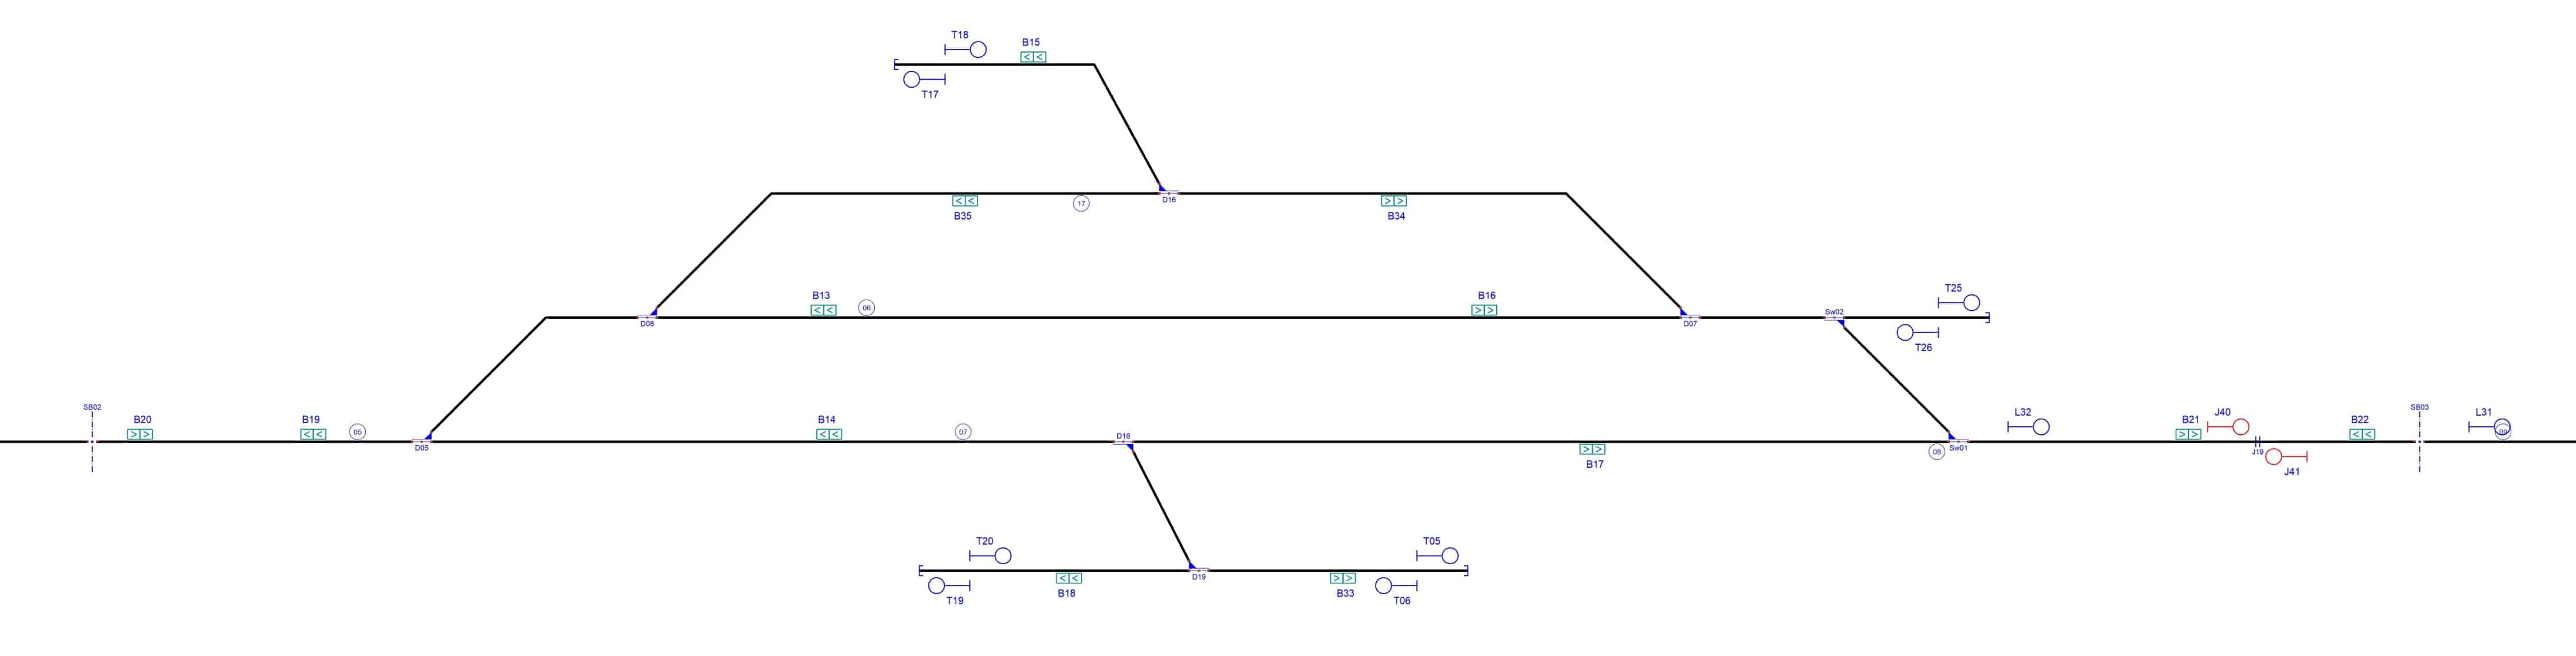
\includegraphics[width=1\textwidth]{resultados-obtenidos/ejemplo4/images/4_step2.png}
        \centering\caption{Señalamiento generado por el RNA para proteger las junturas.}
        %\label{fig:LC_P2}
    \end{figure}

    \begin{figure}[h]
        \centering
        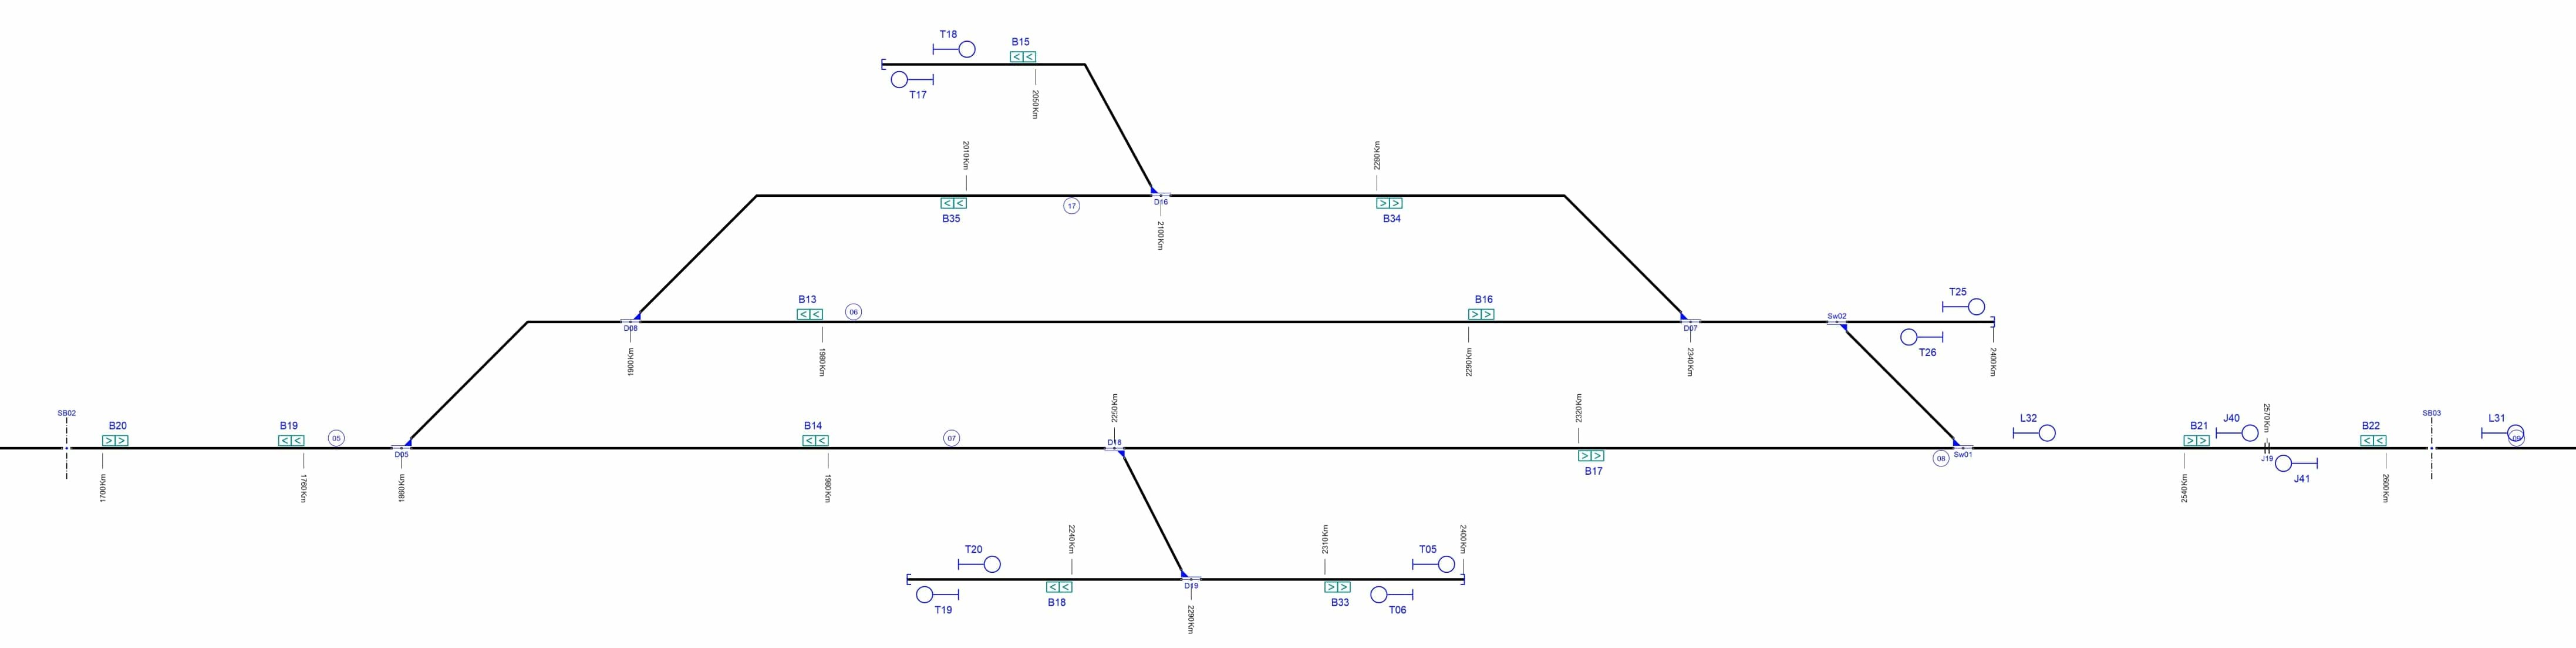
\includegraphics[width=1\textwidth]{resultados-obtenidos/ejemplo4/images/4_step3.png}
        \centering\caption{Señalamiento generado por el RNA para proteger plataformas y cruces de vía.}
        %\label{fig:LC_P2}
    \end{figure}

    \begin{figure}[h]
        \centering
        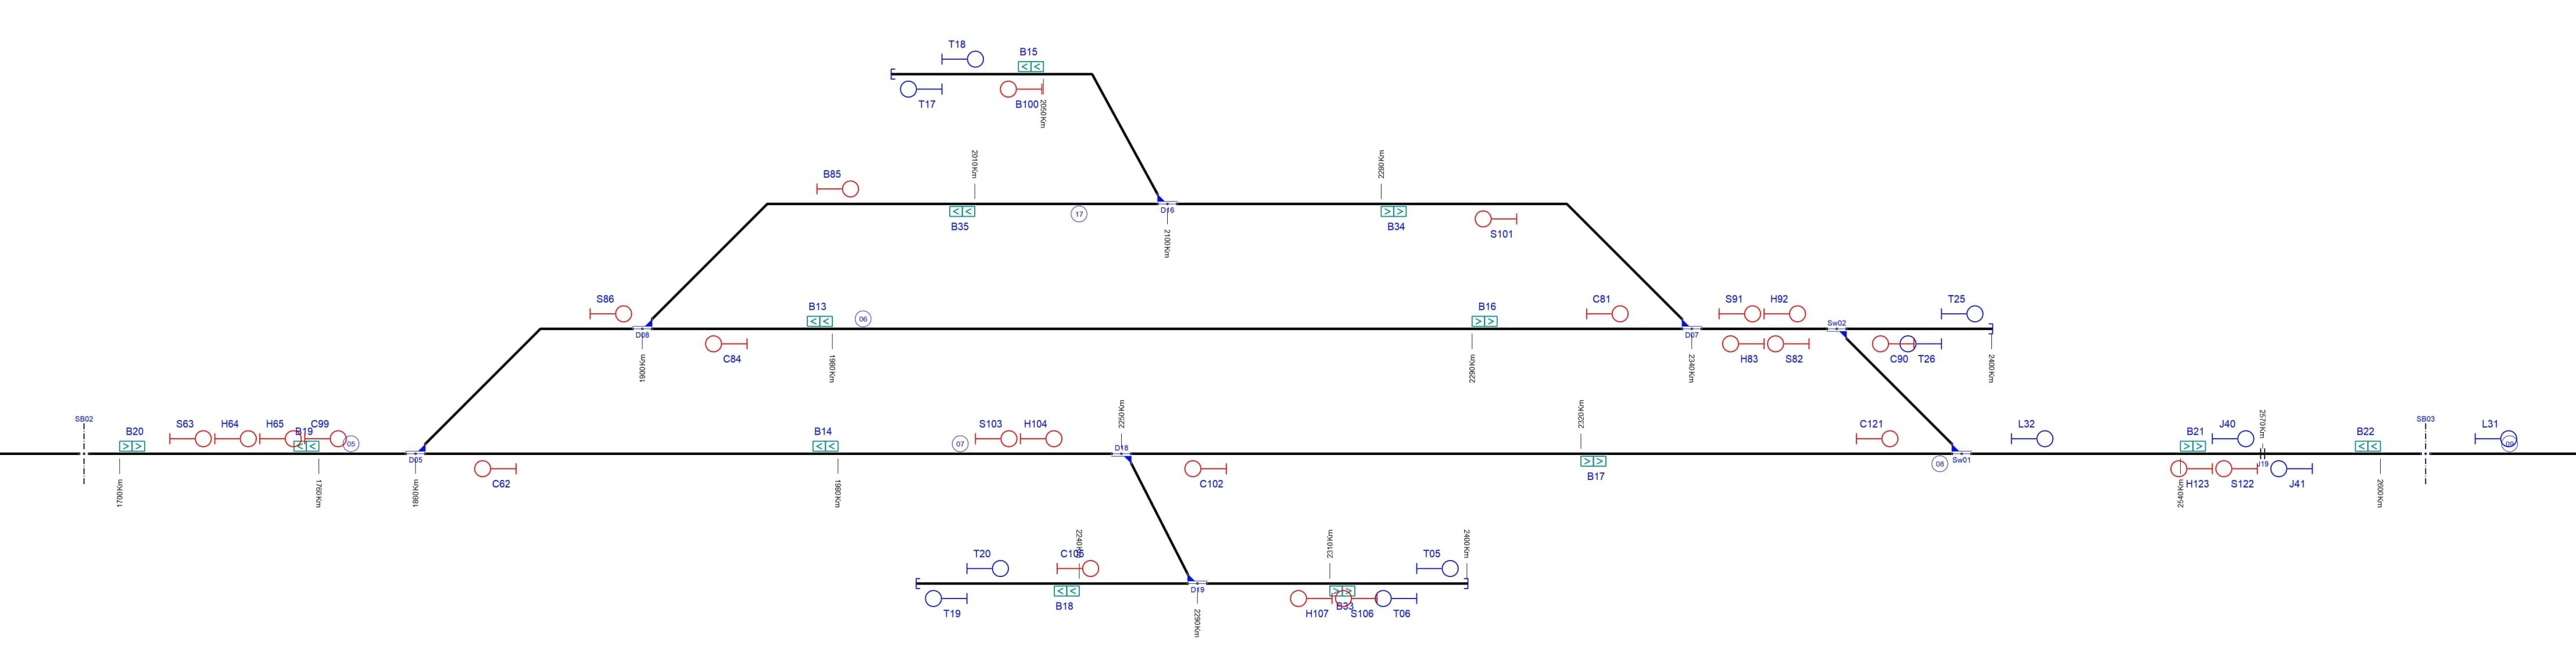
\includegraphics[width=1\textwidth]{resultados-obtenidos/ejemplo4/images/4_step4.png}
        \centering\caption{Señalamiento generado por el RNA para proteger las máquinas de cambios.}
        %\label{fig:LC_P2}
    \end{figure}

    \begin{figure}[h]
        \centering
        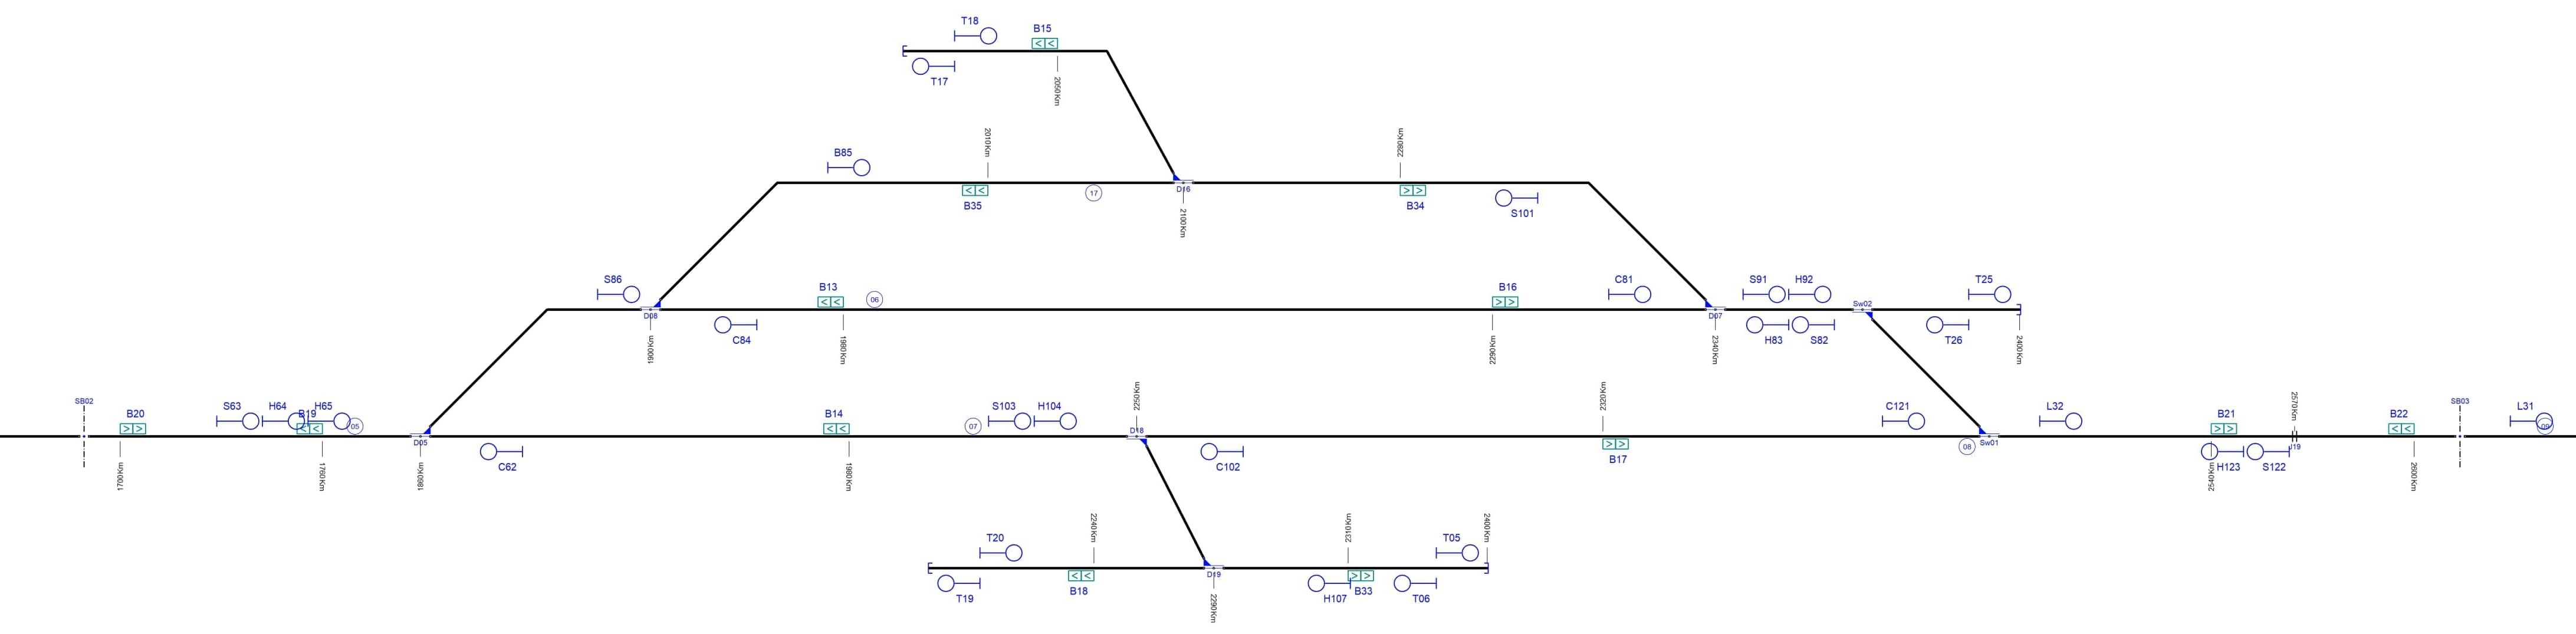
\includegraphics[width=1\textwidth]{resultados-obtenidos/ejemplo4/images/4_RNA.png}
        \centering\caption{Señalamiento generado y simplificado por el RNA.}
        %\label{fig:LC_P2}
    \end{figure}

    \section{Señalamiento original}

    El señalamiento original, ilustrado en la Figura \ref{fig:EJ4_2} incluye 71 señales y es demasiado extenso para describirlo en detalle. El mismo incluye señales de parada próximas a los finales de vías absolutos, señales de partida en las plataformas, señales de protección antes de cada paso a nivel  señales de maniobras antes de converger en una vía principal y señales múltiples para cambios de vías divergentes.
    
    \begin{figure}[H]
    	\centering
    	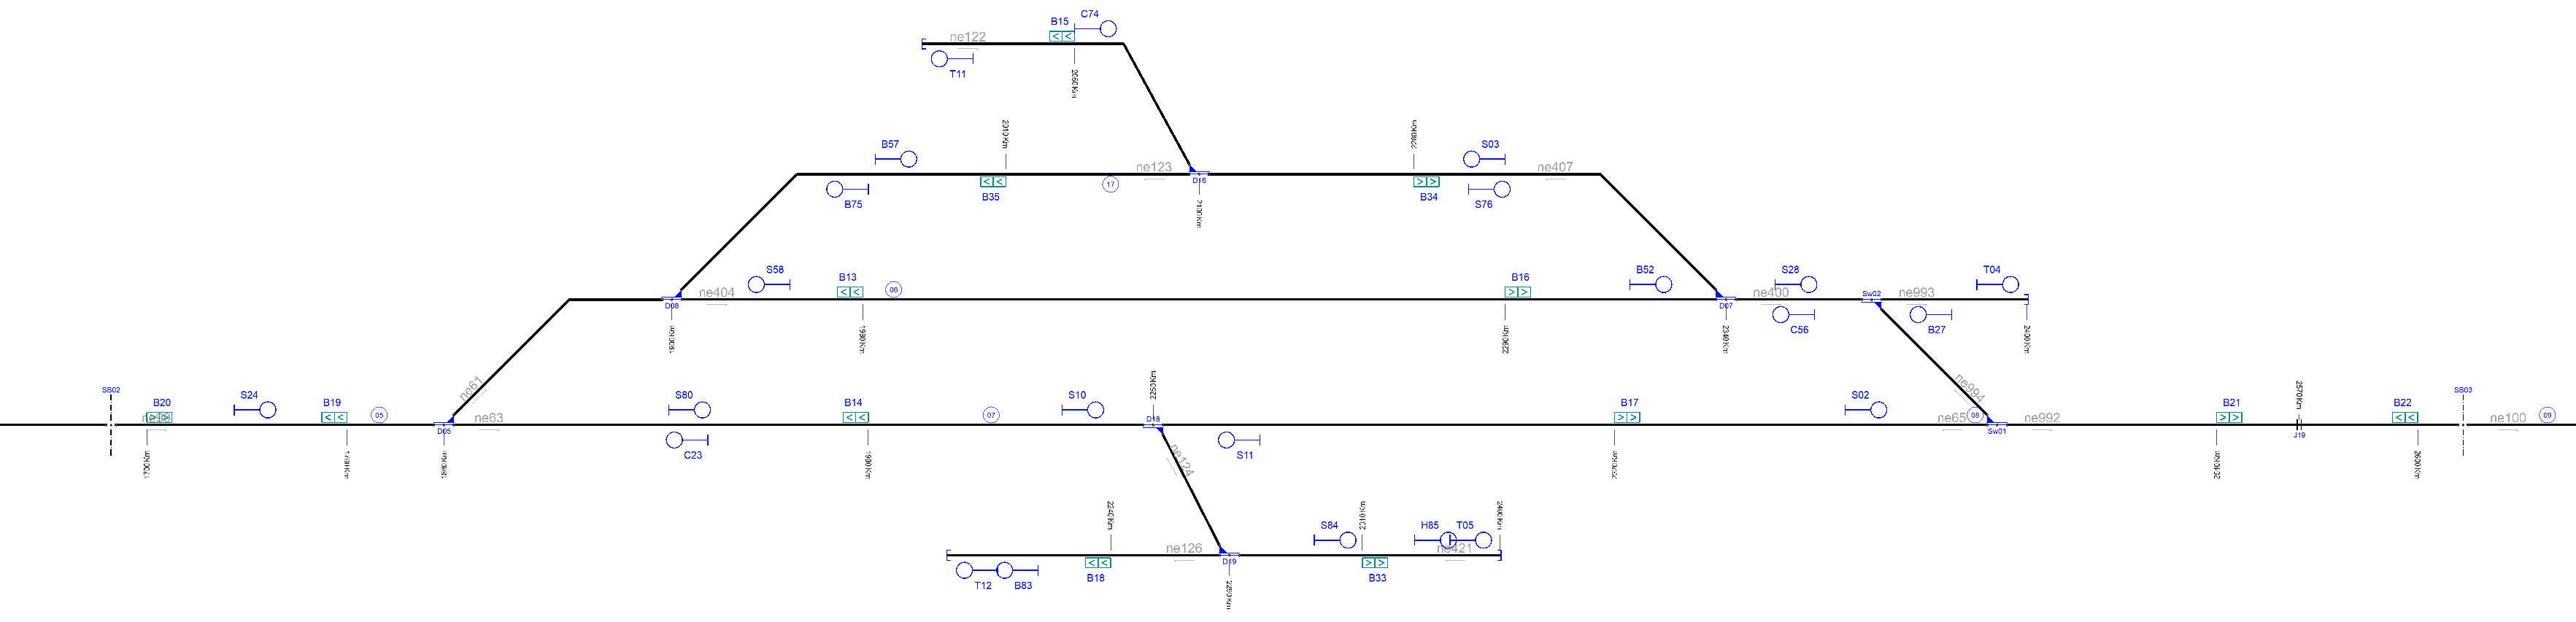
\includegraphics[width=1\textwidth]{resultados-obtenidos/ejemplo4/images/4_original.png}
    	\centering\caption{Señalamiento original del ejemplo 4.}
    	\label{fig:EJ4_2}
    \end{figure}
    
    Estas señales permiten definir hasta un máximo de 77 rutas, las cuales no pueden ser detalladas en una única tabla, por lo que serán particionadas en las Tablas \ref{Tab:tabla_original_4_1}, \ref{Tab:tabla_original_4_2}, \ref{Tab:tabla_original_4_3}, \ref{Tab:tabla_original_4_4} y \ref{Tab:tabla_original_4_5}. En una primera inspección, se puede comprobar que el señalamiento de este ejemplo no es tan complejo como el del ejemplo 3, si es el mas extenso que se analizará en este trabajo.    
    
    \begin{table}[H]
        {
        \caption{Tabla de enclavamiento original del ejemplo 4 (Rutas 1 a 15).}
        \label{Tab:tabla_original_4_1}
        \centering
        \resizebox{1\textwidth}{!}{
            \begin{tabular}{ c c c c c c c }
                \hline	
                    Ruta & Inicio & Final & Cambio & Plataforma & Cruce & netElement \\	
                \hline
                    R$_{01}$ & S$_{15}$ & S$_{24}$ & - & - & Lc$_{02}$ & ne$_{98}$-ne$_{99}$\\
                    R$_{02}$ & S$_{16}$ & S$_{67}$ & Sw$_{04}^{N}$ & - & Lc$_{02}$ & ne$_{98}$-ne$_{292}$\\
                    R$_{03}$ & S$_{16}$ & S$_{43}$ & Sw$_{04}^{R}$ & - & Lc$_{02}$ & ne$_{98}$-ne$_{297}$\\
                    R$_{04}$ & S$_{19}$ & S$_{32}$ & - & - & Lc$_{06}$ & ne$_{100}$-ne$_{101}$\\
                    R$_{05}$ & S$_{20}$ & S$_{11}$ & Sw$_{01}^{N}$ & - & Lc$_{06}$ & ne$_{100}$-ne$_{65}$\\
                    R$_{06}$ & S$_{20}$ & S$_{56}$ & Sw$_{01}^{R}$ & - & Lc$_{06}$ & ne$_{100}$-ne$_{400}$\\
                    R$_{07}$ & S$_{23}$ & S$_{16}$ & - & - & - & ne$_{63}$-ne$_{98}$\\
                    R$_{08}$ & S$_{24}$ & S$_{80}$ & D$_{05}^{N}$ & - & - & ne$_{99}$-ne$_{63}$\\
                    R$_{09}$ & S$_{24}$ & S$_{52}$ & D$_{05}^{R}$-D$_{08}^{N}$ & - & - & ne$_{99}$-ne$_{404}$\\
                    R$_{10}$ & S$_{24}$ & S$_{57}$ & D$_{05}^{R}$-D$_{08}^{R}$ & - & - & ne$_{99}$-ne$_{123}$\\
                    R$_{11}$ & S$_{27}$ & S$_{56}$ & - & - & - & ne$_{993}$-ne$_{400}$\\
                    R$_{12}$ & S$_{28}$ & S$_{04}$ & Sw$_{02}^{N}$ & - & - & ne$_{400}$-ne$_{384}$\\
                    R$_{13}$ & S$_{28}$ & S$_{19}$ & Sw$_{02}^{R}$ & - & Lc$_{05}$ & ne$_{400}$-ne$_{100}$\\
                    R$_{14}$ & S$_{31}$ & S$_{20}$ & - & - & - & ne$_{912}$-ne$_{100}$\\
                    R$_{15}$ & S$_{32}$ & S$_{91}$ & D$_{09}^{N}$ & - & - & ne$_{101}$-ne$_{912}$\\    
                \hline
            \end{tabular}
        }
     }
    \end{table}

	%\lipsum[1]
	
    \begin{table}[H]
        {
        \caption{Tabla de enclavamiento original del ejemplo 4 (Rutas 16 a 30).}
        \label{Tab:tabla_original_4_2}
        \centering
        \resizebox{1\textwidth}{!}{
            \begin{tabular}{ c c c c c c c }
                \hline	
                    Ruta & Inicio & Final & Cambio & Plataforma & Cruce & netElement \\	
                \hline
                    R$_{16}$ & S$_{32}$ & S$_{59}$ & D$_{09}^{R}$-D$_{10}^{N}$ & - & - & ne$_{101}$-ne$_{130}$\\
                    R$_{17}$ & S$_{32}$ & S$_{60}$ & D$_{09}^{R}$-D$_{10}^{R}$ & - & - & ne$_{101}$-ne$_{135}$\\
                    R$_{18}$ & S$_{35}$ & S$_{01}$ & - & - & - & ne$_{290}$-ne$_{130}$\\
                    R$_{19}$ & S$_{39}$ & S$_{43}$ & - & - & - & ne$_{995}$-ne$_{297}$\\
                    R$_{20}$ & S$_{44}$ & S$_{04}$ & - & - & - & ne$_{110}$-ne$_{384}$\\
                    R$_{21}$ & S$_{45}$ & S$_{01}$ & - & - & - & ne$_{295}$-ne$_{130}$\\
                    R$_{22}$ & S$_{46}$ & S$_{63}$ & Sw$_{02}^{N}$ & - & - & ne$_{384}$-ne$_{110}$\\
                    R$_{23}$ & S$_{46}$ & S$_{09}$ & Sw$_{02}^{R}$ & - & - & ne$_{384}$-ne$_{292}$\\
                    R$_{24}$ & S$_{47}$ & S$_{40}$ & - & - & - & ne$_{295}$-ne$_{297}$\\
                    R$_{25}$ & S$_{52}$ & S$_{28}$ & - & - & - & ne$_{404}$-ne$_{400}$\\
                    R$_{26}$ & S$_{56}$ & S$_{58}$ & D$_{07}^{N}$ & - & - & ne$_{400}$-ne$_{404}$\\
                    R$_{27}$ & S$_{56}$ & S$_{03}$ & D$_{07}^{R}$ & - & - & ne$_{400}$-ne$_{407}$\\
                    R$_{28}$ & S$_{57}$ & S$_{76}$ & - & - & - & ne$_{123}$-ne$_{407}$\\
                    R$_{29}$ & S$_{58}$ & S$_{16}$ & - & - & - & ne$_{404}$-ne$_{98}$\\
                    R$_{30}$ & S$_{59}$ & S$_{87}$ & D$_{12}^{T}$ & - & - & ne$_{130}$-ne$_{114}$\\
                \hline
            \end{tabular}
        }
     }
    \end{table}

	%\lipsum[1]
	
    \begin{table}[H]
        {
        \caption{Tabla de enclavamiento original del ejemplo 4 (Rutas 31 a 45).}
        \label{Tab:tabla_original_4_3}
        \centering
        \resizebox{1\textwidth}{!}{
            \begin{tabular}{ c c c c c c c }
                \hline	
                    Ruta & Inicio & Final & Cambio & Plataforma & Cruce & netElement \\	
                \hline
                    R$_{31}$ & S$_{59}$ & S$_{06}$ & D$_{12}^{S}$ & - & - & ne$_{130}$-ne$_{377}$\\
                    R$_{32}$ & S$_{60}$ & S$_{99}$ & - & - & - & ne$_{135}$-ne$_{127}$\\
                    R$_{33}$ & S$_{62}$ & S$_{04}$ & - & - & - & ne$_{104}$-ne$_{384}$\\
                    R$_{34}$ & S$_{63}$ & S$_{01}$ & - & - & - & ne$_{110}$-ne$_{130}$\\
                    R$_{35}$ & S$_{67}$ & S$_{09}$ & - & - & - & ne$_{292}$-ne$_{292}$\\
                    R$_{36}$ & S$_{68}$ & S$_{08}$ & - & - & - & ne$_{290}$-ne$_{290}$\\
                    R$_{37}$ & S$_{74}$ & S$_{76}$ & - & - & - & ne$_{122}$-ne$_{407}$\\
                    R$_{38}$ & S$_{75}$ & S$_{16}$ & - & - & - & ne$_{123}$-ne$_{98}$\\
                    R$_{39}$ & S$_{76}$ & S$_{28}$ & - & - & - & ne$_{407}$-ne$_{400}$\\
                    R$_{40}$ & S$_{80}$ & S$_{10}$ & - & - & - & ne$_{63}$-ne$_{63}$\\
                    R$_{41}$ & S$_{83}$ & S$_{12}$ & - & - & - & ne$_{126}$-ne$_{126}$\\
                    R$_{42}$ & S$_{84}$ & S$_{85}$ & - & - & - & ne$_{421}$-ne$_{421}$\\
                    R$_{43}$ & S$_{85}$ & S$_{05}$ & - & - & - & ne$_{421}$-ne$_{421}$\\
                    R$_{44}$ & S$_{86}$ & S$_{87}$ & - & - & - & ne$_{132}$-ne$_{114}$\\
                    R$_{45}$ & S$_{87}$ & S$_{08}$ & - & - & - & ne$_{114}$-ne$_{290}$\\
                \hline
            \end{tabular}
        }
     }
    \end{table}

	%\lipsum[1]
	
    \begin{table}[H]
        {
        \caption{Tabla de enclavamiento original del ejemplo 4 (Rutas 46 a 160).}
        \label{Tab:tabla_original_4_4}
        \centering
        \resizebox{1\textwidth}{!}{
            \begin{tabular}{ c c c c c c c }
                \hline	
                    Ruta & Inicio & Final & Cambio & Plataforma & Cruce & netElement \\	
                \hline
                    R$_{46}$ & S$_{89}$ & S$_{31}$ & - & - & - & ne$_{132}$-ne$_{912}$\\
                    R$_{47}$ & S$_{90}$ & S$_{89}$ & - & - & - & ne$_{132}$-ne$_{132}$\\
                    R$_{48}$ & S$_{91}$ & S$_{93}$ & - & - & - & ne$_{912}$-ne$_{912}$\\
                    R$_{49}$ & S$_{93}$ & S$_{86}$ & D$_{20}^{N}$ & - & - & ne$_{912}$-ne$_{132}$\\
                    R$_{50}$ & S$_{93}$ & S$_{95}$ & D$_{20}^{R}$ & - & - & ne$_{912}$-ne$_{465}$\\
                    R$_{51}$ & S$_{94}$ & S$_{13}$ & - & - & - & ne$_{133}$-ne$_{133}$\\
                    R$_{52}$ & S$_{95}$ & S$_{96}$ & - & - & - & ne$_{465}$-ne$_{465}$\\
                    R$_{53}$ & S$_{96}$ & S$_{07}$ & - & - & - & ne$_{465}$-ne$_{991}$\\
                    R$_{54}$ & S$_{97}$ & S$_{99}$ & - & - & - & ne$_{134}$-ne$_{127}$\\
                    R$_{55}$ & S$_{98}$ & S$_{20}$ & - & - & - & ne$_{135}$-ne$_{100}$\\
                    R$_{56}$ & S$_{99}$ & S$_{87}$ & D$_{12}^{S}$ & - & - & ne$_{127}$-ne$_{114}$\\
                    R$_{57}$ & S$_{99}$ & S$_{06}$ & D$_{12}^{T}$ & - & - & ne$_{127}$-ne$_{377}$\\
                    R$_{58}$ & S$_{40}$ & S$_{02}$ & Sw$_{03}^{N}$ & - & - & ne$_{297}$-ne$_{65}$\\
                    R$_{59}$ & S$_{40}$ & S$_{15}$ & Sw$_{03}^{R}$ & - & - & ne$_{297}$-ne$_{98}$\\
                    R$_{60}$ & S$_{43}$ & S$_{45}$ & D$_{04}^{N}$ &- & - & ne$_{297}$-ne$_{295}$\\
                \hline
            \end{tabular}
        }
     }
    \end{table}
    
    %\lipsum[1]
    
    \begin{table}[H]
        {
        \caption{Tabla de enclavamiento original del ejemplo 4 (Rutas 61 a 76).}
        \label{Tab:tabla_original_4_5}
        \centering
        \resizebox{1\textwidth}{!}{
            \begin{tabular}{ c c c c c c c }
                \hline	
                    Ruta & Inicio & Final & Cambio & Plataforma & Cruce & netElement \\	
                \hline
                    R$_{61}$ & S$_{43}$ & S$_{46}$ & D$_{04}^{R}$ & - & - & ne$_{297}$-ne$_{384}$\\
                    R$_{62}$ & S$_{01}$ & S$_{20}$ & - & - & - & ne$_{130}$-ne$_{100}$\\
                    R$_{63}$ & S$_{02}$ & S$_{19}$ & - & - & Lc$_{05}$ & ne$_{65}$-ne$_{100}$\\
                    R$_{64}$ & S$_{03}$ & S$_{75}$ & D$_{16}^{N}$ & - & - & ne$_{407}$-ne$_{123}$\\
                    R$_{65}$ & S$_{03}$ & S$_{11}$ & D$_{16}^{R}$ & - & - & ne$_{407}$-ne$_{65}$\\
                    R$_{66}$ & S$_{04}$ & S$_{40}$ & - & - & - & ne$_{384}$-ne$_{297}$\\
                    R$_{67}$ & S$_{06}$ & S$_{10}$ & D$_{15}^{N}$ & - & - & ne$_{377}$-ne$_{63}$\\
                    R$_{68}$ & S$_{06}$ & S$_{35}$ & D$_{15}^{R}$ & - & - & ne$_{377}$-ne$_{290}$\\
                    R$_{69}$ & S$_{07}$ & S$_{68}$ & D$_{01}^{N}$ & - & - & ne$_{991}$-ne$_{290}$\\
                    R$_{70}$ & S$_{07}$ & S$_{47}$ & D$_{01}^{R}$-D$_{03}^{N}$ & - & - & ne$_{991}$-ne$_{295}$\\
                    R$_{71}$ & S$_{07}$ & S$_{44}$ & D$_{01}^{R}$-D$_{03}^{R}$ & - & - & ne$_{991}$-ne$_{110}$\\
                    R$_{72}$ & S$_{08}$ & S$_{15}$ & D$_{14}^{N}$ & - & - & ne$_{290}$-ne$_{98}$\\
                    R$_{73}$ & S$_{08}$ & S$_{03}$ & D$_{14}^{R}$ & - & - & ne$_{290}$-ne$_{407}$\\
                    R$_{74}$ & S$_{09}$ & S$_{35}$ & - & - & - & ne$_{292}$-ne$_{290}$\\
                    R$_{75}$ & S$_{10}$ & S$_{02}$ & D$_{18}^{N}$ & - & - & ne$_{63}$-ne$_{65}$\\
                    R$_{76}$ & S$_{10}$ & S$_{84}$ & D$_{18}^{R}$ & - & - & ne$_{63}$-ne$_{421}$\\
                    R$_{77}$ & S$_{11}$ & S$_{23}$ & - & - & - & ne$_{65}$-ne$_{63}$\\
                \hline
            \end{tabular}
        }
     }
    \end{table}
    
    Algunas rutas abarcan mas de un \textit{netElement}, como por ejemplo la ruta R75 que comienza en la señal S10 y finaliza en la señal S02, atravesando los \textit{netElements} ne63 y ne65, utilizando el cambio de vías D18 en posición reversa.
    \section{Señalamiento generado por el RNA}

    El RNA también exporta la misma información mostrada en el Código \ref{lst:EJ4_8} en una hoja de cálculo, similar a la que se visualiza en las Tablas \ref{Tab:tabla_generated_4_1}, \ref{Tab:tabla_generated_4_2}, \ref{Tab:tabla_generated_4_3}, \ref{Tab:tabla_generated_4_4}, \ref{Tab:tabla_generated_4_5} y \ref{Tab:tabla_generated_4_6}.

    \begin{table}[H]
        {
        \caption{Tabla de enclavamiento del ejemplo 4 generada por el RNA (Rutas 1 a 15).}
        \label{Tab:tabla_generated_4_1}
        \centering
        \resizebox{1\textwidth}{!}{
            \begin{tabular}{ c c c c c c c }
                \hline	
                    Ruta & Inicio & Final & Cambio & Plataforma & Cruce & netElement \\	
                \hline
                    R$_{01}$ & T$_{02}$ & S$_{71}$ &  &  &  & ne$_{991}$-ne$_{991}$\\
                    R$_{02}$ & T$_{04}$ & J$_{35}$ & D$_{14}^{R}$-D$_{15}^{R}$ &  &  & ne$_{377}$-ne$_{290}$\\
                    R$_{03}$ & T$_{04}$ & T$_{15}$ & D$_{15}^{N}$ &  &  & ne$_{377}$-ne$_{113}$\\
                    R$_{04}$ & T$_{06}$ & C$_{62}$ & D$_{18}^{R}$-D$_{19}^{R}$ &  &  & ne$_{421}$-ne$_{63}$\\
                    R$_{05}$ & T$_{06}$ & T$_{19}$ & D$_{19}^{N}$ &  &  & ne$_{421}$-ne$_{126}$\\
                    R$_{06}$ & T$_{08}$ & S$_{119}$ &  &  &  & ne$_{450}$-ne$_{127}$\\
                    R$_{07}$ & T$_{08}$ & C$_{87}$ &  &  &  & ne$_{450}$-ne$_{130}$\\
                    R$_{08}$ & T$_{10}$ & J$_{45}$ & D$_{20}^{R}$-D$_{21}^{R}$ &  &  & ne$_{465}$-ne$_{912}$\\
                    R$_{09}$ & T$_{10}$ & T$_{21}$ & D$_{21}^{N}$ &  &  & ne$_{465}$-ne$_{133}$\\
                    R$_{10}$ & T$_{12}$ & S$_{109}$ &  &  &  & ne$_{102}$-ne$_{114}$\\
                    R$_{11}$ & T$_{14}$ & S$_{125}$ & D$_{04}^{R}$ &  &  & ne$_{104}$-ne$_{297}$\\
                    R$_{12}$ & T$_{16}$ & T$_{03}$ & D$_{15}^{N}$ &  &  & ne$_{113}$-ne$_{377}$\\
                    R$_{13}$ & T$_{18}$ & S$_{91}$ & D$_{07}^{R}$-D$_{16}^{R}$ &  &  & ne$_{122}$-ne$_{400}$\\
                    R$_{14}$ & T$_{20}$ & T$_{05}$ & D$_{19}^{N}$ &  &  & ne$_{126}$-ne$_{421}$\\
                    R$_{15}$ & T$_{22}$ & T$_{09}$ & D$_{21}^{N}$ &  &  & ne$_{133}$-ne$_{465}$\\
                \hline
            \end{tabular}
        }
     }
    \end{table}

	%\lipsum[1]
	
    \begin{table}[H]
        {
        \caption{Tabla de enclavamiento del ejemplo 4 generada por el RNA (Rutas 16 a 30).}
        \label{Tab:tabla_generated_4_2}
        \centering
        \resizebox{1\textwidth}{!}{
            \begin{tabular}{ c c c c c c c }
                \hline	
                    Ruta & Inicio & Final & Cambio & Plataforma & Cruce & netElement \\	
                \hline
                    R$_{16}$ & T$_{24}$ & S$_{105}$ & D$_{24}^{R}$ &  &  & ne$_{134}$-ne$_{127}$\\
                    R$_{17}$ & L$_{29}$ & J$_{48}$ &  &  &  & ne$_{114}$-ne$_{114}$\\
                    R$_{18}$ & S$_{30}$ & X$_{50}$ &  &  &  & ne$_{98}$-ne$_{98}$\\
                    R$_{19}$ & L$_{31}$ & X$_{52}$ &  &  &  & ne$_{100}$-ne$_{100}$\\
                    R$_{20}$ & J$_{35}$ & T$_{01}$ & D$_{01}^{N}$ &  &  & ne$_{290}$-ne$_{991}$\\
                    R$_{21}$ & J$_{36}$ & J$_{38}$ & Sw$_{04}^{N}$ &  &  & ne$_{292}$-ne$_{996}$\\
                    R$_{22}$ & J$_{37}$ & J$_{35}$ & D$_{14}^{N}$ &  &  & ne$_{292}$-ne$_{290}$\\
                    R$_{23}$ & J$_{38}$ & S$_{30}$ &  &  &  & ne$_{996}$-ne$_{98}$\\
                    R$_{24}$ & J$_{40}$ & L$_{31}$ &  &  &  & ne$_{992}$-ne$_{100}$\\
                    R$_{25}$ & J$_{43}$ & X$_{53}$ &  &  &  & ne$_{101}$-ne$_{100}$\\
                    R$_{26}$ & J$_{45}$ & J$_{43}$ & D$_{09}^{N}$ &  &  & ne$_{912}$-ne$_{101}$\\
                    R$_{27}$ & J$_{46}$ & L$_{29}$ & D$_{23}^{N}$ &  &  & ne$_{132}$-ne$_{114}$\\
                    R$_{28}$ & J$_{47}$ & J$_{45}$ & D$_{20}^{N}$ &  &  & ne$_{132}$-ne$_{912}$\\
                    R$_{29}$ & J$_{48}$ & T$_{11}$ &  &  &  & ne$_{114}$-ne$_{102}$\\
                    R$_{30}$ & X$_{50}$ & S$_{55}$ &  &  & Lc$_{01}$ & ne$_{98}$-ne$_{99}$\\
                \hline
            \end{tabular}
        }
     }
    \end{table}

	%\lipsum[1]
	
    \begin{table}[H]
        {
        \caption{Tabla de enclavamiento del ejemplo 4 generada por el RNA (Rutas 31 a 45).}
        \label{Tab:tabla_generated_4_3}
        \centering
        \resizebox{1\textwidth}{!}{
            \begin{tabular}{ c c c c c c c }
                \hline	
                    Ruta & Inicio & Final & Cambio & Plataforma & Cruce & netElement \\	
                \hline
                    R$_{31}$ & X$_{51}$ & S$_{127}$ &  &  & Lc$_{01}$ & ne$_{98}$-ne$_{996}$\\
                    R$_{32}$ & X$_{52}$ & S$_{59}$ &  &  & Lc$_{04}$ & ne$_{100}$-ne$_{101}$\\
                    R$_{33}$ & X$_{53}$ & S$_{121}$ &  &  & Lc$_{04}$ & ne$_{100}$-ne$_{992}$\\
                    R$_{34}$ & C$_{54}$ & X$_{51}$ & D$_{05}^{N}$ & & & ne$_{63}$-ne$_{98}$\\
                    R$_{35}$ & S$_{55}$ & S$_{79}$ & D$_{05}^{R}$ &  &  & ne$_{99}$-ne$_{61}$\\
                    R$_{36}$ & S$_{55}$ & S$_{96}$ & D$_{05}^{N}$ &  &  & ne$_{99}$-ne$_{63}$\\
                    R$_{37}$ & S$_{59}$ & S$_{111}$ & D$_{09}^{N}$ &  &  & ne$_{101}$-ne$_{912}$\\
                    R$_{38}$ & S$_{59}$ & S$_{82}$ & D$_{09}^{R}$ &  &  & ne$_{101}$-ne$_{910}$\\
                    R$_{39}$ & S$_{64}$ & S$_{69}$ & D$_{01}^{R}$ &  &  & ne$_{991}$-ne$_{288}$\\
                    R$_{40}$ & S$_{64}$ & S$_{87}$ & D$_{01}^{N}$ &  &  & ne$_{991}$-ne$_{290}$\\
                    R$_{41}$ & C$_{67}$ & T$_{01}$ & D$_{01}^{R}$-D$_{03}^{N}$ &  &  & ne$_{295}$-ne$_{991}$\\
                    R$_{42}$ & B$_{68}$ & S$_{124}$ & D$_{04}^{R}$ &  &  & ne$_{110}$-ne$_{297}$\\
                    R$_{43}$ & S$_{69}$ & C$_{70}$ & D$_{03}^{N}$ &  &  & ne$_{288}$-ne$_{295}$\\
                    R$_{44}$ & S$_{69}$ & B$_{68}$ & D$_{03}^{R}$ &  &  & ne$_{288}$-ne$_{110}$\\
                    R$_{45}$ & C$_{70}$ & S$_{124}$ & D$_{04}^{N}$ &  &  & ne$_{295}$-ne$_{297}$\\
                \hline
            \end{tabular}
        }
     }
    \end{table}
    
    %\lipsum[1]

    \begin{table}[H]
        {
        \caption{Tabla de enclavamiento del ejemplo 4 generada por el RNA (Rutas 46 a 60).}
        \label{Tab:tabla_generated_4_4}
        \centering
        \resizebox{1\textwidth}{!}{
            \begin{tabular}{ c c c c c c c }
                \hline	
                    Ruta & Inicio & Final & Cambio & Plataforma & Cruce & netElement \\	
                \hline
                    R$_{46}$ & B$_{71}$ & T$_{13}$ &  &  &  & ne$_{384}$-ne$_{104}$\\
                    R$_{47}$ & B$_{71}$ & T$_{01}$ & D$_{01}^{R}$-D$_{03}^{R}$ &  &  & ne$_{384}$-ne$_{991}$\\
                    R$_{48}$ & S$_{72}$ & C$_{67}$ & D$_{04}^{N}$ &  &  & ne$_{297}$-ne$_{295}$\\
                    R$_{49}$ & S$_{72}$ & B$_{71}$ & D$_{04}^{R}$ &  &  & ne$_{297}$-ne$_{384}$\\
                    R$_{50}$ & C$_{74}$ & S$_{84}$ & D$_{07}^{N}$ &  &  & ne$_{404}$-ne$_{400}$\\
                    R$_{51}$ & S$_{75}$ & C$_{77}$ & D$_{07}^{N}$ &  &  & ne$_{400}$-ne$_{404}$\\
                    R$_{52}$ & S$_{75}$ & S$_{94}$ & D$_{07}^{R}$ &  &  & ne$_{400}$-ne$_{407}$\\
                    R$_{53}$ & C$_{77}$ & X$_{51}$ & D$_{05}^{R}$-D$_{08}^{N}$ &  &  & ne$_{404}$-ne$_{98}$\\
                    R$_{54}$ & B$_{78}$ & S$_{84}$ & D$_{07}^{R}$-D$_{16}^{N}$ &  &  & ne$_{123}$-ne$_{400}$\\
                    R$_{55}$ & S$_{79}$ & C$_{74}$ & D$_{08}^{N}$ &  &  & ne$_{61}$-ne$_{404}$\\
                    R$_{56}$ & S$_{79}$ & B$_{78}$ & D$_{08}^{R}$ &  &  & ne$_{61}$-ne$_{123}$\\
                    R$_{57}$ & C$_{80}$ & J$_{43}$ & D$_{09}^{R}$-D$_{10}^{N}$ &  &  & ne$_{130}$-ne$_{101}$\\
                    R$_{58}$ & B$_{81}$ & S$_{105}$ & D$_{24}^{N}$ &  &  & ne$_{135}$-ne$_{127}$\\
                    R$_{59}$ & S$_{82}$ & S$_{108}$ & D$_{10}^{N}$ &  &  & ne$_{910}$-ne$_{130}$\\
                    R$_{60}$ & S$_{82}$ & B$_{81}$ & D$_{10}^{R}$ &  &  & ne$_{910}$-ne$_{135}$\\
                \hline
            \end{tabular}
        }
     }
    \end{table}

	%\lipsum[1]
	
    \begin{table}[H]
        {
        \caption{Tabla de enclavamiento del ejemplo 4 generada por el RNA (Rutas 61 a 75).}
        \label{Tab:tabla_generated_4_5}
        \centering
        \resizebox{1\textwidth}{!}{
            \begin{tabular}{ c c c c c c c }
                \hline	
                    Ruta & Inicio & Final & Cambio & Plataforma & Cruce & netElement \\	
                \hline
					R$_{61}$ & C$_{83}$ & S$_{75}$ & Sw$_{02}^{N}$ &  &  & ne$_{993}$-ne$_{400}$\\
                    R$_{62}$ & S$_{84}$ & T$_{25}$ & Sw$_{02}^{N}$ &  &  & ne$_{400}$-ne$_{993}$\\
                    R$_{63}$ & S$_{84}$ & J$_{40}$ & Sw$_{02}^{R}$-Sw$_{01}^{R}$ &  &  & ne$_{400}$-ne$_{992}$\\
                    R$_{64}$ & S$_{87}$ & J$_{36}$ & D$_{14}^{N}$ &  &  & ne$_{290}$-ne$_{292}$\\
                    R$_{65}$ & S$_{87}$ & T$_{03}$ & D$_{14}^{R}$-D$_{15}^{R}$ &  &  & ne$_{290}$-ne$_{377}$\\
                    R$_{66}$ & S$_{94}$ & T$_{17}$ & D$_{16}^{R}$ &  &  & ne$_{407}$-ne$_{122}$\\
                    R$_{67}$ & S$_{94}$ & X$_{51}$ & D$_{05}^{R}$-D$_{08}^{R}$-D$_{16}^{N}$ &  &  & ne$_{407}$-ne$_{98}$\\
                    R$_{68}$ & C$_{95}$ & C$_{54}$ & D$_{18}^{N}$ &  &  & ne$_{65}$-ne$_{63}$\\
                    R$_{69}$ & S$_{96}$ & C$_{120}$ & D$_{18}^{N}$ &  &  & ne$_{63}$-ne$_{65}$\\
                    R$_{70}$ & S$_{96}$ & T$_{05}$ & D$_{18}^{R}$-D$_{19}^{R}$ &  &  & ne$_{63}$-ne$_{421}$\\
                    R$_{71}$ & S$_{102}$ & J$_{47}$ & D$_{23}^{N}$ &  &  & ne$_{114}$-ne$_{132}$\\
                    R$_{72}$ & S$_{102}$ & S$_{118}$ & D$_{23}^{R}$-D$_{12}^{RR}$ &  &  & ne$_{114}$-ne$_{127}$\\
                    R$_{73}$ & S$_{102}$ & C$_{80}$ & D$_{23}^{R}$-D$_{12}^{NR}$ &  &  & ne$_{114}$-ne$_{130}$\\
                    R$_{74}$ & S$_{105}$ & L$_{29}$ & D$_{23}^{R}$-D$_{12}^{RR}$ &  &  & ne$_{912}$-ne$_{465}$\\
                    R$_{75}$ & S$_{105}$ & T$_{07}$ & D$_{12}^{RN}$ &  &  & ne$_{912}$-ne$_{132}$\\
                \hline
            \end{tabular}
        }
     }
    \end{table}
    
    %\lipsum[1]
    
    \begin{table}[H]
        {
        \caption{Tabla de enclavamiento del ejemplo 4 generada por el RNA (Rutas 76 a 89).}
        \label{Tab:tabla_generated_4_6}
        \centering
        \resizebox{1\textwidth}{!}{
            \begin{tabular}{ c c c c c c c }
                \hline	
                    Ruta & Inicio & Final & Cambio & Plataforma & Cruce & netElement \\	
                \hline
                 	R$_{76}$ & S$_{108}$ & L$_{29}$ & D$_{23}^{R}$-D$_{12}^{NR}$ &  &  & ne$_{130}$-ne$_{114}$\\
                 	R$_{77}$ & S$_{108}$ & T$_{07}$ & D$_{12}^{NN}$ &  &  & ne$_{130}$-ne$_{450}$\\
                    R$_{78}$ & S$_{111}$ & T$_{09}$ & D$_{20}^{R}$-D$_{21}^{R}$ &  &  & ne$_{912}$-ne$_{465}$\\
                    R$_{79}$ & S$_{111}$ & J$_{46}$ & D$_{20}^{N}$ &  &  & ne$_{912}$-ne$_{132}$\\
                    R$_{80}$ & S$_{118}$ & J$_{43}$ & D$_{09}^{R}$-D$_{10}^{R}$-D$_{24}^{N}$ &  &  & ne$_{127}$-ne$_{101}$\\
                    R$_{81}$ & S$_{118}$ & T$_{23}$ & D$_{24}^{R}$ &  &  & ne$_{127}$-ne$_{134}$\\
                    R$_{82}$ & C$_{120}$ & J$_{40}$ & Sw$_{01}^{N}$ &  &  & ne$_{65}$-ne$_{992}$\\
                    R$_{83}$ & S$_{121}$ & C$_{95}$ & Sw$_{01}^{N}$ &  &  & ne$_{992}$-ne$_{65}$\\
                    R$_{84}$ & S$_{121}$ & S$_{75}$ & Sw$_{02}^{R}$-Sw$_{01}^{R}$ &  &  & ne$_{992}$-ne$_{400}$\\
                    R$_{85}$ & C$_{123}$ & S$_{72}$ & Sw$_{03}^{N}$ &  &  & ne$_{995}$-ne$_{297}$\\
                    R$_{86}$ & S$_{124}$ & T$_{27}$ & Sw$_{03}^{N}$ &  &  & ne$_{297}$-ne$_{995}$\\
                    R$_{87}$ & S$_{124}$ & J$_{38}$ & Sw$_{03}^{R}$-Sw$_{04}^{R}$ &  &  & ne$_{297}$-ne$_{996}$\\
                    R$_{88}$ & S$_{128}$ & J$_{37}$ & Sw$_{04}^{N}$ &  &  & ne$_{996}$-ne$_{292}$\\
                    R$_{89}$ & S$_{128}$ & S$_{72}$ & Sw$_{03}^{R}$-Sw$_{04}^{R}$ &  &  & ne$_{996}$-ne$_{297}$\\
                \hline
            \end{tabular}
        }
     }
    \end{table}
    
    En una primera inspección podemos ver que el nuevo señalamiento tiene 89 rutas, versus las 77 rutas del señalamiento original (ver Tabla \ref{Tab:tabla_original_4}). Esto se debe a que muchas de las rutas generadas son particiones de las rutas originales, al ser demasiado extensas o abarcar demasiados elementos ferroviarios sin paradas intermedias.
    \subsection{Sistema generado por el ACG}
	
	En base a la red de grafos, ilustrada en la Figura \ref{fig:EJ4_8}, el ACG determinó la siguiente cantidad de elementos, tal puede visualizarse en el Código \ref{lst:EJ4_8}.

	\begin{lstlisting}[language = {}, caption = Cantidad de elementos a implementar por el ACG, label = {lst:EJ4_8}]
	n_netElements:47
	n_switch:21
	n_doubleSwitch:1
	n_borders:5
	n_buffers:14
	n_levelCrossings:2
	n_platforms:0
	n_scissorCrossings:0
	n_signals:77
	N : 315
	M : 268
	\end{lstlisting}

	El código VHDL generado por el ACG es importado en un proyecto de Vivado, donde es sintetizado e implementado para generar el bitstream que será utilizado para programar la FPGA. La cantidad de elementos de la FPGA utilizados por el sistema post-síntesis y post-implementación, así como el porcentaje de uso de la plataforma, son detallados en la Tabla \ref{Tab:tabla_ACG_4}.
	
	\begin{table}[H]
		{
			\caption{Síntesis e implementación del ejemplo 4 generado por el ACG.}
			\label{Tab:tabla_ACG_4}
			\centering
			%\small
			%\centering
			\begin{center}
				\resizebox{0.7\textwidth}{!}{
					\begin{tabular}{ c c c c }
						\hline	
						Recursos & Síntesis & Implementación & Uso \\	
						\hline
						LUT & 13589 & 13556 & 25.54-25.48\%\\
						FF & 17256 & 17256 & 16.22\%\\
						IO & 16 & 16 & 12.80\%\\
						BUFG & 1 & 1 & 3.13\%\\
						\hline
					\end{tabular}
				}
			\end{center}
		}    
	\end{table}
	
	En este ejemplo, la cantidad de recursos utilizados es baja y el tiempo de sintetización e implementación es de 1 minuto con 39 segundos y 1 minuto con 22 segundos respectivamente.
    \subsection{Validacion del sistema}

    \lipsum[1]

    \begin{table}[!h]
        {
        \caption{Equivalencias entre las rutas 1 a 15 originales y las generadas por el RNA.}
        \label{Tab:tabla_validation_4_1}
        \centering
        %\small
            %\centering
            \begin{center}
            \resizebox{1\textwidth}{!}{
            \begin{tabular}{ c c c c }
                \hline	
                    Original & Señales & RNA & Señales \\	
                \hline
                    R$_{01}$ & S$_{15}$-S$_{24}$ & R$_{31}$ & S$_{52}$-S$_{63}$\\
                    R$_{02}$ & S$_{16}$-S$_{67}$ & R$_{32}$+R$_{89}$ & S$_{53}$-S$_{37}$\\
                    R$_{03}$ & S$_{16}$-S$_{43}$ & R$_{32}$+R$_{90}$ & S$_{53}$-S$_{79}$\\
                    R$_{04}$ & S$_{19}$-S$_{32}$ & R$_{35}$ & S$_{60}$-S$_{67}$\\
                    R$_{05}$ & S$_{20}$-S$_{11}$ & R$_{34}$+R$_{84}$ & S$_{59}$-S$_{102}$\\
                    R$_{06}$ & S$_{20}$-S$_{56}$ & R$_{34}$+R$_{85}$ & S$_{59}$-S$_{82}$\\
                    R$_{07}$ & S$_{23}$-S$_{16}$ & R$_{37}$ & S$_{62}$-S$_{53}$\\
                    R$_{08}$ & S$_{24}$-S$_{80}$ & R$_{39}$ & S$_{63}$-S$_{103}$\\
                    R$_{09}$ & S$_{24}$-S$_{52}$ & R$_{38}$+R$_{58}$ & S$_{63}$-S$_{81}$\\
                    R$_{10}$ & S$_{24}$-S$_{57}$ & R$_{38}$+R$_{59}$ & S$_{63}$-S$_{85}$\\
                    R$_{11}$ & S$_{27}$-S$_{56}$ & R$_{66}$ & S$_{90}$-S$_{82}$\\
                    R$_{12}$ & S$_{28}$-S$_{04}$ & R$_{54}$+R$_{56}$+R$_{32}$+R$_{90}$+R$_{52}$ & S$_{82}$-S$_{78}$\\
                    R$_{13}$ & S$_{28}$-S$_{19}$ & R$_{68}$+R$_{25}$ & S$_{91}$-S$_{31}$\\
                    R$_{14}$ & S$_{31}$-S$_{20}$ & R$_{27}$+R$_{26}$ & S$_{45}$-S$_{61}$\\
                    R$_{15}$ & S$_{32}$-S$_{91}$ & R$_{40}$ & S$_{67}$-S$_{112}$\\                 
                \hline
            \end{tabular}
            }
            \end{center}
        }    
    \end{table}

    \begin{table}[!h]
        {
        \caption{Equivalencias entre las rutas 16 a 30 originales y las generadas por el RNA.}
        \label{Tab:tabla_validation_4_2}
        \centering
        %\small
            %\centering
            \begin{center}
            \resizebox{1\textwidth}{!}{
            \begin{tabular}{ c c c c }
                \hline	
                    Original & Señales & RNA & Señales \\	
                \hline
                    R$_{16}$ & S$_{32}$-S$_{59}$ & R$_{41}$+R$_{63}$+R$_{78}$ & S$_{67}$-S$_{87}$\\
                    R$_{17}$ & S$_{32}$-S$_{60}$ & R$_{41}$+R$_{65}$ & S$_{67}$-S$_{88}$\\
                    R$_{18}$ & S$_{35}$-S$_{01}$ & R$_{69}$+R$_{22}$+R$_{24}$+R$_{31}$+R$_{39}$+R$_{74}$+R$_{83}$+R$_{25}$+R$_{35}$+R$_{41}$+R$_{63}$+R$_{78}$ & S$_{94}$-S$_{87}$\\
                    R$_{19}$ & S$_{39}$-S$_{43}$ & R$_{86}$ & S$_{124}$-S$_{79}$\\
                    R$_{20}$ & S$_{44}$-S$_{04}$ & R$_{45}$+R$_{52}$ & S$_{75}$-S$_{78}$\\
                    R$_{21}$ & S$_{45}$-S$_{01}$ & R$_{48}$+R$_{88}$+R$_{24}$+R$_{31}$+R$_{39}$+R$_{74}$+R$_{83}$+R$_{25}$+R$_{35}$+R$_{41}$+R$_{63}$+R$_{78}$ & S$_{77}$-S$_{87}$\\
                    R$_{22}$ & S$_{46}$-S$_{63}$ & R$_{50}$+R$_{42}$+R$_{47}$ & S$_{78}$-S$_{75}$\\
                    R$_{23}$ & S$_{46}$-S$_{09}$ & R$_{50}$+R$_{43}$+R$_{69}$ & S$_{78}$-S$_{36}$\\
                    R$_{24}$ & S$_{47}$-S$_{40}$ & R$_{48}$ & S$_{77}$-S$_{125}$\\
                    R$_{25}$ & S$_{52}$-S$_{28}$ & R$_{53}$ & S$_{81}$-S$_{91}$\\
                    R$_{26}$ & S$_{56}$-S$_{58}$ & R$_{54}$ & S$_{82}$-S$_{84}$\\
                    R$_{27}$ & S$_{56}$-S$_{03}$ & R$_{55}$ & S$_{82}$-S$_{101}$\\
                    R$_{28}$ & S$_{57}$-S$_{76}$ & R$_{57}$+R$_{55}$ & S$_{85}$-S$_{101}$\\
                    R$_{29}$ & S$_{58}$-S$_{16}$ & R$_{56}$ & S$_{84}$-S$_{53}$\\
                    R$_{30}$ & S$_{59}$-S$_{87}$ & R$_{60}$+R$_{41}$+R$_{63}$ & S$_{87}$-S$_{29}$\\              
                \hline
            \end{tabular}
            }
            \end{center}
        }    
    \end{table}

    \begin{table}[!h]
        {
        \caption{Equivalencias entre las rutas 31 a 45 originales y las generadas por el RNA.}
        \label{Tab:tabla_validation_4_3}
        \centering
        %\small
            %\centering
            \begin{center}
            \resizebox{1\textwidth}{!}{
            \begin{tabular}{ c c c c }
                \hline	
                    Original & Señales & RNA & Señales \\	
                \hline
                    R$_{31}$ & S$_{59}$-S$_{06}$ & R$_{60}$+R$_{26}$+R$_{34}$+R$_{84}$+R$_{73}$+R$_{37}$+R$_{32}$+R$_{89}$+R$_{23}$+R$_{70}$ & S$_{87}$-S$_{03}$\\
                    R$_{32}$ & S$_{60}$-S$_{99}$ & R$_{61}$+R$_{77}$ & S$_{88}$-S$_{119}$\\
                    R$_{33}$ & S$_{62}$-S$_{04}$ & R$_{11}$+R$_{52}$ & S$_{14}$-S$_{78}$\\
                    R$_{34}$ & S$_{63}$-S$_{01}$ & R$_{45}$+R$_{88}$+R$_{24}$+R$_{31}$+R$_{39}$+R$_{74}$+R$_{83}$+R$_{35}$+R$_{35}$+R$_{41}$+R$_{63}$+R$_{78}$ & S$_{75}$-S$_{87}$\\
                    R$_{35}$ & S$_{67}$-S$_{09}$ & R$_{89}$ & S$_{128}$-S$_{37}$\\
                    R$_{36}$ & S$_{68}$-S$_{08}$ & R$_{43}$ & S$_{71}$-S$_{94}$\\
                    R$_{37}$ & S$_{74}$-S$_{76}$ & R$_{13}$+R$_{55}$ & S$_{18}$-S$_{101}$\\
                    R$_{38}$ & S$_{75}$-S$_{16}$ & R$_{57}$+R$_{54}$+R$_{56}$ & S$_{85}$-S$_{53}$\\
                    R$_{39}$ & S$_{76}$-S$_{28}$ & R$_{71}$+R$_{13}$ & S$_{101}$-S$_{91}$\\
                    R$_{40}$ & S$_{80}$-S$_{10}$ & R$_{31}$+R$_{39}$ & S$_{52}$-S$_{103}$\\
                    R$_{41}$ & S$_{83}$-S$_{12}$ & R$_{05}$ & S$_{06}$-S$_{19}$\\
                    R$_{42}$ & S$_{84}$-S$_{85}$ & R$_{75}$ & S$_{103}$-S$_{05}$\\
                    R$_{43}$ & S$_{85}$-S$_{05}$ & R$_{75}$ & S$_{103}$-S$_{05}$\\
                    R$_{44}$ & S$_{86}$-S$_{87}$ & R$_{28}$ & S$_{46}$-S$_{29}$\\
                    R$_{45}$ & S$_{87}$-S$_{08}$ & R$_{77}$+R$_{81}$+R$_{26}$+R$_{34}$+R$_{84}$+R$_{73}$+R$_{37}$+R$_{32}$+R$_{89}$+R$_{23}$ & S$_{109}$-S$_{35}$\\              
                \hline
            \end{tabular}
            }
            \end{center}
        }    
    \end{table}

    \begin{table}[!h]
        {
        \caption{Equivalencias entre las rutas 46 a 60 originales y las generadas por el RNA.}
        \label{Tab:tabla_validation_4_4}
        \centering
        %\small
            %\centering
            \begin{center}
            \resizebox{1\textwidth}{!}{
            \begin{tabular}{ c c c c }
                \hline	
                    Original & Señales & RNA & Señales \\	
                \hline
                    R$_{46}$ & S$_{89}$-S$_{31}$ & R$_{29}$ & S$_{47}$-S$_{45}$\\
                    R$_{47}$ & S$_{90}$-S$_{89}$ & R$_{76}$ & S$_{109}$-S$_{47}$\\
                    R$_{48}$ & S$_{91}$-S$_{93}$ & R$_{40}$ & S$_{67}$-S$_{112}$\\
                    R$_{49}$ & S$_{93}$-S$_{86}$ & R$_{80}$ & S$_{112}$-S$_{46}$\\
                    R$_{50}$ & S$_{93}$-S$_{95}$ & R$_{79}$ & S$_{112}$-S$_{09}$\\
                    R$_{51}$ & S$_{94}$-S$_{13}$ & R$_{09}$ & S$_{10}$-S$_{21}$\\
                    R$_{52}$ & S$_{95}$-S$_{96}$ & R$_{79}$ & S$_{112}$-S$_{09}$\\
                    R$_{53}$ & S$_{96}$-S$_{07}$ & R$_{08}$+R$_{27}$+R$_{26}$+R$_{34}$+R$_{84}$+R$_{73}$+R$_{37}$+R$_{32}$+R$_{89}$+R$_{23}$+R$_{21}$ & S$_{10}$-S$_{01}$\\
                    R$_{54}$ & S$_{97}$-S$_{99}$ & R$_{16}$+R$_{77}$ & S$_{24}$-S$_{119}$\\
                    R$_{55}$ & S$_{98}$-S$_{20}$ & R$_{61}$+R$_{77}$+R$_{81}$+R$_{26}$ & S$_{88}$-S$_{61}$\\
                    R$_{56}$ & S$_{99}$-S$_{87}$ & R$_{82}$+R$_{16}$ & S$_{119}$-S$_{29}$\\
                    R$_{57}$ & S$_{99}$-S$_{06}$ & R$_{81}$+R$_{26}$+R$_{34}$+R$_{84}$+R$_{73}$+R$_{37}$+R$_{32}$+R$_{89}$+R$_{23}$+R$_{70}$& S$_{119}$-S$_{03}$\\
                    R$_{58}$ & S$_{40}$-S$_{02}$ & R$_{88}$+R$_{24}$+R$_{31}$+R$_{39}$+R$_{74}$ & S$_{125}$-S$_{121}$\\
                    R$_{59}$ & S$_{40}$-S$_{15}$ & R$_{88}$+R$_{24}$ & S$_{125}$-S$_{30}$\\
                    R$_{60}$ & S$_{43}$-S$_{45}$ & R$_{51}$ & S$_{87}$-S$_{43}$\\              
                \hline
            \end{tabular}
            }
            \end{center}
        }    
    \end{table}

    \begin{table}[!h]
        {
        \caption{Equivalencias entre las rutas 61 a 77 originales y las generadas por el RNA.}
        \label{Tab:tabla_validation_4_5}
        \centering
        %\small
            %\centering
            \begin{center}
            \resizebox{1\textwidth}{!}{
            \begin{tabular}{ c c c c }
                \hline	
                    Original & Señales & RNA & Señales \\	
                \hline
                    R$_{61}$ & S$_{43}$-S$_{46}$ & R$_{52}$ & S$_{79}$-S$_{78}$\\
                    R$_{62}$ & S$_{01}$-S$_{20}$ & R$_{60}$+R$_{26}$ & S$_{87}$-S$_{43}$\\
                    R$_{63}$ & S$_{02}$-S$_{19}$ & R$_{83}$+R$_{25}$ & S$_{121}$-S$_{31}$\\
                    R$_{64}$ & S$_{03}$-S$_{75}$ & R$_{72}$+R$_{31}$+R$_{38}$+R$_{59}$ & S$_{101}$-S$_{85}$\\
                    R$_{65}$ & S$_{03}$-S$_{11}$ & R$_{71}$+R$_{13}$+R$_{68}$+R$_{84}$ & S$_{101}$-S$_{102}$\\
                    R$_{66}$ & S$_{04}$-S$_{40}$ & R$_{49}$+R$_{11}$ & S$_{78}$-S$_{125}$\\
                    R$_{67}$ & S$_{06}$-S$_{10}$ & R$_{02}$+R$_{69}$+R$_{22}$+R$_{24}$+R$_{31}$+R$_{39}$ & S$_{04}$-S$_{103}$\\
                    R$_{68}$ & S$_{06}$-S$_{35}$ & R$_{02}$ & S$_{04}$-S$_{35}$\\
                    R$_{69}$ & S$_{07}$-S$_{68}$ & R$_{43}$ & S$_{71}$-S$_{94}$\\
                    R$_{70}$ & S$_{07}$-S$_{47}$ & R$_{42}$+R$_{46}$ & S$_{71}$-S$_{77}$\\
                    R$_{71}$ & S$_{07}$-S$_{44}$ & R$_{42}$+R$_{47}$ & S$_{71}$-S$_{75}$\\
                    R$_{72}$ & S$_{08}$-S$_{15}$ & R$_{69}$+R$_{22}$+R$_{24}$ & S$_{94}$-S$_{30}$\\
                    R$_{73}$ & S$_{08}$-S$_{03}$ & R$_{69}$+R$_{22}$+R$_{24}$+R$_{31}$+R$_{38}$+R$_{58}$+R$_{53}$+R$_{55}$ & S$_{94}$-S$_{101}$\\
                    R$_{74}$ & S$_{09}$-S$_{35}$ & R$_{23}$ & S$_{37}$-S$_{35}$\\
                    R$_{75}$ & S$_{10}$-S$_{02}$ & R$_{74}$ & S$_{103}$-S$_{121}$\\
                    R$_{76}$ & S$_{10}$-S$_{84}$ & R$_{75}$ & S$_{103}$-S$_{05}$\\
                    R$_{77}$ & S$_{11}$-S$_{23}$ & R$_{73}$ & S$_{102}$-S$_{62}$\\            
                \hline
            \end{tabular}
            }
            \end{center}
        }    
    \end{table}